\documentclass[a4paper,12pt]{article}
\usepackage{amsfonts}
\usepackage[centertags]{amsmath}
\usepackage{amssymb}
\usepackage{amsthm}
\usepackage{fixmath,multirow}
\usepackage{float}
\usepackage{framed}
\usepackage{graphicx}
\usepackage{hyperref}
\usepackage[justification=centering]{caption}
\usepackage[numbers]{natbib}
\usepackage{subcaption}
\usepackage[normalem]{ulem}
\usepackage{url}
\usepackage{xcolor,lipsum}
\usepackage{xcolor,colortbl}
\usepackage{minted}
\usepackage{fancyvrb}
\usepackage{verbatim}
\usepackage{ifthen}
\usepackage{dirtytalk}
\usepackage{tcolorbox}
\usepackage[framemethod=TikZ]{mdframed}
\usepackage{booktabs}
\setlength{\parindent}{4ex}
\usepackage{siunitx}


\title{\textbf{Classification of Alzheimer's Disease using Machine Learning on Plasma Proteomic Biomarkers}}
\author{\textbf{Daniel Jones}}
\begin{document}
\maketitle
\pagenumbering{gobble}
\begin{center}
    Student Reference Number: 10691995
\end{center}
\begin{center}
    
\includegraphics[scale = 0.4]{Pics/shield.png}
\end{center}
\begin{center}
    MSc Health Data Science and Statistics
\end{center}
\begin{center}
    School of Engineering, Computing and Mathematics \\ University of Plymouth
\end{center}
\begin{center}
    Supervisor - Dr Shakil Awan
\end{center}

\section*{Acknowledgements}

I’d like to thank Dr. Shakil Awan for supervising this project. His guidance, expertise, and significant research in the field have been invaluable, and this project has been a fantastic opportunity to deepen my understanding of disease prediction with machine learning algorithms.

I’d also like to thank Hamza Bhatti for sharing his extensive knowledge of GFET methodologies and machine learning techniques, which played a key role in shaping the research and helping me bring it to life.

\section*{Abstract}
\label{abstract}

Alzheimer’s disease (AD) is the leading cause of dementia worldwide, yet current diagnostic pathways rely heavily on invasive, costly, or inaccessible methods such as cerebrospinal fluid analysis and positron emission tomography imaging. This study explores the potential of plasma proteomic biomarkers, analysed with machine learning (ML), to provide a minimally invasive and scalable alternative for AD diagnosis. Proteomic and clinical data from the Alzheimer’s Disease Neuroimaging Initiative (ADNI) were preprocessed and modelled using three algorithms: support vector machines (SVM), extreme gradient boosting (XGBoost), and a feed-forward neural network (NeuralNet). Model performance was evaluated on a held-out test set using accuracy, macro F1, AUROC, and AUPRC metrics. All models demonstrated strong predictive ability, with XGBoost achieving the highest performance (AUROC $\approx$ 0.94, AUPRC $\approx$ 0.97) when restricted to the top-10 most informative features. SVM also performed competitively, particularly with feature reduction, while the neural network showed potential but required larger datasets for greater stability. Feature importance analyses revealed biologically relevant biomarkers associated with immune regulation, lipid metabolism, and neuronal integrity, aligning with existing literature and highlighting potential novel candidates. These findings support the feasibility of blood-based, ML-driven diagnostic tools for AD, offering a foundation for future clinical validation and integration with emerging biosensing platforms to enable accessible, early detection.

\newpage
\pagenumbering{roman}
\vspace*{-2cm}\tableofcontents

\newpage
\listoffigures\label{listoffigures}
\addcontentsline{toc}{section}{List of Figures}

\newpage
\listoftables\label{listoftables}
\addcontentsline{toc}{section}{List of Tables}

\newpage\pagenumbering{arabic}
\section{Introduction}
Dementia is an umbrella term for a range of neurocognitive syndromes characterised by a progressive decline in cognitive function, including memory, thinking, and reasoning, often severe enough to interfere with daily life. It is not a specific disease but rather a general term describing the symptoms of cognitive impairment. The most prevalent cause of dementia is Alzheimer's disease (AD), a specific neurodegenerative disorder that accounts for an estimated 60-80\% of all dementia cases \cite{better2023alzheimer}. AD is defined by distinct neuropathological hallmarks, primarily the extracellular accumulation of amyloid-beta plaques and the intracellular formation of neurofibrillary tangles composed of hyperphosphorylated tau protein \cite{deture2019neuropathological}. These pathologies lead to synaptic dysfunction, neuronal loss, and brain atrophy, resulting in the irreversible cognitive and functional decline in patients. The progressive nature of AD outlines the importance of early detection. Identifying the disease in its early stages, before significant and widespread neurodegeneration has occurred, provides the best opportunity to implement therapeutic interventions, manage symptoms, and potentially slow disease progression, thereby preserving quality of life for as long as possible.

Dementia represents a profound and escalating challenge in modern healthcare, with around 57 million people suffering globally as of 2021 and AD contributing to 60 to 70 percent of those cases \cite{WHO2025dementia}. As the most common form of dementia, it contributes to a significant global health crisis, with projections indicating that the number of affected individuals will nearly triple by 2050 \cite{nichols2022estimation}. The societal and economic burden is immense, including direct medical costs estimated in the hundreds of billions annually, extensive long-term care needs, as well as the emotional and physical toll on patients, families, and caregivers \cite{wimo2023worldwide}. The diagnostic journey for AD is often a prolonged and demanding process, with current clinical pathways frequently taking up to two years to reach a definitive conclusion \cite{bungon2021graphene}. The current diagnostic path relies on a combination of methods, including cerebrospinal fluid (CSF) analysis via invasive lumbar puncture, costly positron emission tomography (PET) imaging, and subjective cognitive assessments, that come with limitations \cite{olsson2016csf}. These primary methods are not only time-consuming but also hindered by accessibility issues, with high costs and the need for specialised medical centres making them inaccessible to many patients. Consequently, individuals often experience significant delays in receiving a diagnosis and appropriate interventions, which can exacerbate disease progression and place further strain on an already overstretched healthcare system.

The urgent need for a paradigm shift in AD diagnostics is therefore undeniable. An ideal solution would be efficient, cost-effective, scalable, and minimally invasive, allowing for widespread screening and earlier detection. It is within this context that blood-based biomarkers have emerged as a frontier of intense research \cite{scholl2024challenges}. Blood is a readily accessible biological medium, and its collection is a routine, cost-effective clinical procedure. Advances in proteomic technologies now allow for the high-throughput analysis of hundreds of proteins from a single plasma sample, offering a window into the complex pathophysiological processes underlying AD, including amyloid and tau pathology, neuroinflammation, and synaptic dysfunction. The challenge, however, lies in interpreting the intricate patterns within this complex data to find a reliable \say{proteomic signature} of the disease.

This is where Machine Learning (ML) presents a transformative opportunity. Esteva et. al. show how convolutional neural networks are capable of performing dermatologist-level classifications of skin cancer, just one example of machine learning success in the healthcare world \cite{esteva2017dermatologist}. The application of ML in creating generalised, biomarker-driven models for AD diagnosis remains underutilised. ML algorithms are uniquely suited to identify subtle, non-linear patterns within complex datasets like proteomics, patterns that are often undetected by traditional statistical analysis. This dissertation proposes the development and validation of such a ML-based diagnostic model, designed specifically to analyse multiple subsets of blood-based protein biomarkers associated with AD. By leveraging the comprehensive, longitudinal data from the Alzheimer's Disease Neuroimaging Initiative (ADNI) \cite{adni_biofluid_biomarker}, this approach aims to provide a proof-of-concept for a non-invasive, rapid, and accessible diagnostic alternative.

This research seeks to bridge a notable gap in the literature by evaluating the feasibility of an AI-driven diagnostic tool for AD. The primary aim of this dissertation is to develop and validate a machine learning model capable of accurately classifying individuals based on their plasma protein profiles. To achieve this, the study will first involve the meticulous processing and preparation of the ADNI plasma proteomics and corresponding clinical datasets to make them suitable for machine learning analysis. This study will employ cross-validation techniques to make sure the model is well-generalised. Following this, the research will utilise advanced feature selection techniques to identify the most notable protein biomarkers for distinguishing between diagnostic groups. Multiple machine learning algorithms will then be trained, tested, and systematically compared to determine the optimal architecture for the diagnostic classification task. The final model's efficacy will be evaluated using standard metrics of diagnostic accuracy, including sensitivity, specificity, and the area under the receiver operating characteristic curve (AUC), thereby providing a comprehensive assessment of its potential clinical utility.

Through rigorous model development and validation, this dissertation aspires to contribute both to academic research and future clinical practice. By demonstrating the potential of a blood-based, AI-powered diagnostic tool, this work provides a foundation for the future integration of such solutions in AD detection. Ultimately, by enabling earlier and more accessible diagnosis, this research aims to improve patient outcomes and support a more efficient, equitable, and data-driven approach to managing many neurodegenerative diseases like AD.

\newpage
\section{Literature Review}


Having outlined the clinical urgency, research motivation, and methodological goals of this study, this section provides a critical overview of the current literature relevant to the development of a machine learning-based diagnostic model for AD. The review is structured around five key areas: (1) the limitations of conventional diagnostic methods; (2) the emergence of blood-based biomarkers and their role in early AD detection; (3) the application of machine learning in biomarker analysis and diagnostic modelling; (4) the role of biosensor technologies, particularly graphene-based platforms, in real-time biomarker detection; and (5) ongoing challenges related to standardisation, reproducibility, and clinical translation. This foundation supports the methodological design of the present study and highlights key knowledge gaps that this dissertation aims to address.



\subsection{Conventional Diagnostic Methods for AD and Their Limitations}
\textbf{Cognitive assessments.} The initial screening for AD often relies on cognitive tests and mental status examinations. Instruments such as the Mini-Mental State Examination (MMSE) and the Montreal Cognitive Assessment (MoCA) are widely used to detect cognitive impairment \cite{folstein1975mini, nasreddine2005montreal}. While these tests are inexpensive and non-invasive, their accuracy in early AD is limited due to the subtle nature of some cognitive decline \cite{petersen1999mild, albert2013diagnosis}. Moreover, cognitive test performance can be influenced by a patient’s educational background and language/cultural factors, which affect reliability \cite{ramos2025education}. For example, tasks involving reading, writing, or arithmetic on standard dementia screens tend to disadvantage individuals with lower formal education, potentially leading to under-diagnosis in those populations \cite{ramos2025education}. Conversely, patients with high cognitive reserve (often correlated with higher education) might score within normal ranges until later in the disease, yielding false negatives \cite{stern2012cognitive}. In short, cognitive exams alone are not definitive – they must be interpreted in context and are often supplemented by biomarker or imaging tests for a conclusive diagnosis.

\textbf{Neuroimaging.} Structural imaging with Magnetic Resonance Imaging (MRI) and functional or molecular imaging with Positron Emission Tomography (PET) provides valuable information about AD pathology \cite{jack2018nia, gelosa2012prognostic}. MRI can reveal patterns of brain atrophy, such as hippocampal volume loss, a common characteristic of AD \cite{jack2018nia}. Alongside this, PET can detect abnormal protein accumulations; for instance, amyloid PET imaging visualises amyloid-$\beta$ plaques, and tau PET scans can visualise tau tangles in the brain \cite{gelosa2012prognostic}. Fluorodeoxyglucose Positron Emission Tomography (FDG-PET) is also used to measure regional brain metabolism, which typically decreases in AD \cite{huseby2022blood}. These neuroimaging techniques significantly improve diagnostic accuracy when positive \cite{jack2018nia, huseby2022blood}. However, they come with drawbacks. PET imaging requires specialised facilities and is generally an expensive option, which limits accessibility \cite{gelosa2012prognostic}. PET also exposes patients to a small amount of ionising radiation, which carries a small risk of causing other health issues. MRI is more widely available and non-invasive, but a suitable MRI for dementia can still be costly and likely requires expert analysis \cite{jack2018nia}. Additionally, MRI changes in early AD may not be specific or obvious; many elderly individuals without dementia show some brain atrophy similar to that of early AD \cite{jack2018nia}. Overall, while imaging is a powerful tool, its high cost and limited availability make it impractical for routine early screening of every at-risk individual. Reliance on imaging can contribute to diagnostic delays and inequities in access.

\textbf{Cerebrospinal fluid (CSF) biomarkers.} Analysis of CSF obtained via lumbar puncture provides direct biochemical evidence of AD presence \cite{blennow2009csf}. The established CSF biomarkers for AD are amyloid-beta 42 (A$\beta$42), total tau (T-tau), and phosphorylated tau (P-tau). In AD, CSF A$\beta$42 is typically reduced (reflecting deposition of amyloid plaques in the brain), while T-tau and P-tau are elevated (reflecting neurofibrillary tangle pathology and neuronal damage) \cite{blennow2009csf, olsson2016csf}. These markers have shown excellent diagnostic performance in distinguishing AD from cognitively normal controls \cite{olsson2016csf}. For example, a meta-analysis reported that CSF T-tau is on average ~2.5 times higher in AD than controls, and P-tau ~1.9 times higher, while A$\beta$42 is about half the level of controls \cite{olsson2016csf}. Clinically, a combination of low A$\beta$42 and high tau in CSF is considered highly indicative of AD, even at the mild cognitive impairment stage \cite{olsson2016csf}. The drawback, however, is that obtaining CSF requires a lumbar puncture, which is an invasive procedure that many patients are reluctant to undergo \cite{blennow2009csf}. Lumbar puncture can cause discomfort, headaches, and rarely more serious complications, limiting its acceptance for routine screening. Furthermore, performing and analysing CSF tests demand medical expertise and infrastructure that may not be available outside specialised centres \cite{blennow2009csf}. These factors make CSF biomarker testing less accessible and not easily scalable as a mass screening tool. There are also pre-analytical variability issues (differences in collection and storage of data) that historically hindered widespread standardisation \cite{jammeh2016identification}. In summary, while CSF biomarkers are highly informative for AD, their invasiveness and logistical requirements motivate the search for less invasive methods such as blood-based biomarker analysis.


\subsection{Emerging Blood-Based Biomarkers for Early AD Detection}
Blood-based biomarkers have garnered significant attention as a potential solution for scalable, non-invasive, and cost-effective Alzheimer's disease (AD) diagnostics \cite{jammeh2016identification, palmqvist2020discriminative}. Blood collection is routine in clinical practice, making it ideal for early screening. However, detecting AD pathology in blood is challenging due to the blood–brain barrier and the dilution of central biomarkers \cite{hampel2018blood}. Despite this, advances in assay sensitivity have enabled detection of proteins like phosphorylated tau (p-tau) and neurofilament light (NfL), both of which correlate with AD-related neurodegeneration and have shown promise in distinguishing AD from other dementias \cite{olsson2016csf, palmqvist2020discriminative}.

Among emerging candidates, \textbf{clusterin (apolipoprotein J)} has been repeatedly implicated in AD pathology. It plays key roles in inflammation, lipid transport, and amyloid-beta clearance \cite{foster2019clusterin}. Genome-wide association studies identify the CLU gene as a strong genetic risk factor for late-onset AD \cite{milinkeviciute2023clusterin}. Elevated plasma clusterin levels have been associated with brain atrophy and cognitive decline, and postmortem studies show that clusterin accumulates at synapses—especially in individuals carrying the APOE $\epsilon$4 allele \cite{jackson2019clusterin}. Its measurable presence in plasma and its mechanistic role in AD progression make it a promising biomarker, with high-sensitivity assays and biosensors now enabling detection at sub-picogram levels \cite{foster2019clusterin}.

\textbf{Apolipoprotein E4 (APOE4)} is widely recognised as the strongest genetic risk factor for late-onset Alzheimer’s disease \cite{corder1993gene}. Carrying the $\epsilon$4 allele increases a person’s risk by two to twelve times, depending on whether they have one or two copies \cite{bilousova2019apolipoprotein}. APOE4 status is usually determined through genetic testing rather than by measuring the protein directly. It is commonly used to help assess disease risk and to select participants for clinical trials. Some blood-based diagnostic models include APOE as a predictive factor, and research is underway to develop biosensors that can detect ApoE protein variants in blood samples \cite{bungon2021graphene}.

Due to the limitations of individual biomarkers, multi-analyte blood panels are being explored. A panel developed by Jammeh et al. \cite{jammeh2016identification} using ADNI data combined six plasma proteins—A1M, A2M, AAT, ApoE, complement C3, and pancreatic polypeptide—with age to classify AD with 85.4\% sensitivity and 78.6\% specificity. This study highlighted that panels capturing different biological pathways can enhance diagnostic performance. However, reproducibility remains a concern. Biomarker combinations often vary between studies due to cohort differences, assay techniques, and statistical overfitting, impeding clinical translation \cite{hampel2018blood}.

Emerging omics technologies and transcriptomics further extend the biomarker landscape. For example, Sood et al. \cite{sood2015novel} reported a multi-tissue RNA signature that correlates with cognitive health, suggesting systemic gene expression changes could signal early neurodegeneration. As omics datasets grow, the need for computational methods to extract meaningful patterns becomes more pressing \cite{eteleeb2024brain}.

In summary, blood-based biomarkers are a promising route for earlier, scalable AD detection. Proteins like clusterin, genetic factors like APOE4, and combined biomarker panels have shown encouraging results \cite{hampel2018blood}. Nonetheless, variability and lack of standardisation hinder their immediate clinical use \cite{hampel2018blood}. Machine learning offers a path forward—refining biomarker selection and integrating diverse features into robust, generalisable diagnostic models \cite{winchester2023artificial}.

\subsection{Machine Learning Approaches in AD Diagnosis}
Machine learning (ML) offers powerful tools for developing diagnostic models for Alzheimer’s disease (AD), especially when working with large, complex datasets such as those generated by biomarker studies \cite{winchester2023artificial}. Unlike traditional statistical approaches that assess one or a few variables at a time, ML methods can analyse many features at once, detect subtle patterns, and capture non-linear relationships \cite{khosravi2023demystifying, arya2023systematic}. This makes them particularly useful in AD research, where weak signals from blood proteins, genetic factors, and clinical variables may together indicate disease presence. This section summarises how ML is applied to AD diagnostics, with a focus on feature selection, classification models, and transcriptomic approaches.

Feature selection is essential when dealing with many potential biomarkers. Including too many variables can lead to overfitting and make models difficult to interpret or use in clinical settings \cite{saeys2007review}. ML techniques can help identify the most relevant features. For example, Jammeh et al. \cite{jammeh2016identification} used ML to narrow down a panel of six plasma proteins that showed good accuracy for detecting AD. In another study, Huseby et al. \cite{huseby2022blood} applied a Random Forest algorithm to blood transcriptomic data and selected a small set of genes that reliably distinguished AD from other conditions. The top-ranked genes were related to basic cellular functions, suggesting widespread biological effects in AD. Feature selection not only improves model performance but also helps reveal underlying disease mechanisms.

Classification models such as Random Forest (RF), Linear Discriminant Analysis (LDA), support vector machines (SVM), and logistic regression have all been used to classify individuals as AD or non-AD. In Huseby et al.'s study, an RF model trained on gene expression data achieved an AUC of around 0.82 \cite{huseby2022blood}. LDA produced similar results and was used to validate the selected features. Other studies have shown classification accuracies between 75–85\%, depending on the data and algorithms used \cite{winchester2023artificial}.

More advanced models that utilise deep learning, including convolutional neural networks (CNNs), are widely used for analysing imaging data like MRI or PET scans \cite{malik2024deep}. In one study, an AlexNet-based CNN achieved 95\% accuracy in classifying AD from MRI images \cite{el2024novel}. Despite this, their performance and interpretability are still under evaluation in clinical practice. Deep learning has also been applied to biomarker data in some studies, including time-series data to predict AD progression \cite{nguyen2020predicting}. However, such models often require large datasets to perform well, making them less practical for smaller blood biomarker datasets unless data is pooled across studies.

Transcriptomic and RNA-based approaches provide another layer of diagnostic information. Gene expression changes in blood can reflect systemic effects of AD. Huseby et al. used ML on RNA data to classify AD and other neurodegenerative diseases, showing comparable or better performance than protein-based models \cite{huseby2022blood}. Sood et al. \cite{sood2015novel} developed a multi-tissue RNA signature of healthy ageing, which correlated with cognitive performance and may help flag early cognitive decline.

ML is also well suited to combining different data types—clinical features, proteins, RNA, genetics—into a single model \cite{li2021applied,ren2025artificial}. For example, a model might take in a person’s age, APOE genotype, protein biomarker levels, and transcriptomic data to produce an AD risk score. This integrative approach has been shown to improve accuracy and offers a path toward more robust, personalised diagnostics \cite{huseby2022blood}.

In summary, ML is becoming a central tool in AD biomarker research. It helps identify the most informative markers, builds accurate classifiers, and integrates diverse data types. While results are promising, models still need thorough validation on independent datasets to ensure reliability and generalisability.


\subsection{Integrating Machine Learning with Biosensor Technology for Point-of-Care Diagnostics}
A rapidly developing, futuristic approach to AD diagnosis combines advanced biosensors with ML algorithms for rapid, point-of-care testing.  In this model, a patient provides a small blood sample, which is immediately analysed by a sensitive biosensor measuring one or more biomarkers. The results are processed on-site or via the cloud using an ML model, yielding an interpretable AD risk score within minutes. Graphene field-effect transistor (GFET) biosensors are among the most promising technologies for this purpose: they have demonstrated detection of Alzheimer’s biomarkers (such as clusterin) down to femtogram levels \cite{bungon2021graphene}; they offer high sensitivity, multiplexing capability, and compatibility with point-of-care platforms \cite{krishnan2023graphene}; and aptamer-modified GFET systems have even been patented for wireless, at-home testing of AD biomarkers \cite{ono2024challenges}.

Graphene FET biosensors: Graphene, a monolayer of carbon atoms, posseses remarkable electrical and material properties that make it highly suitable as a sensing substrate. \cite{novoselov2004electric}. GFET biosensors typically consist of a graphene channel between transistor electrodes; when biomolecules (such as a specific protein) bind to receptors on the graphene surface, they induce changes in electrical conductance that can be measured. Graphene’s high conductivity and large surface area allow it to detect biomolecule binding events with very high sensitivity, often without the need for any fluorescent or radioactive labels \cite{ohno2010label}. In the context of AD, GFET sensors have been developed to detect biomarkers like amyloid-beta, tau, and clusterin \cite{krishnan2023graphene}. Bungon et al. (2021) reported the fabrication of a GFET biosensor for the AD protein Clusterin, demonstrating an impressive limit of detection (LoD) of ~300 femtograms per millilitre (fg/mL) (approximately $4 \times 10^{-15}$ M) for clusterin in solution \cite{bungon2021graphene}. This means the sensor could reliably detect clusterin at concentrations down to the picogram range, showing enough capability to measure typical concentrations in human blood, indicating excellent sensitivity. They achieved linear detection of clusterin across a range of 1 to 100 pg/mL \cite{bungon2021graphene}. Moreover, the sensor was shown to be quite specific; when exposed to a much higher concentration of an unrelated protein (human chorionic gonadotropin, used as a control), it showed minimal cross-reactive signal \cite{bungon2021graphene}. These results are very promising for a point-of-care AD test: clusterin in plasma could conceivably be detected with just a drop of blood and without extensive sample processing.

A major advantage of GFET and similar biosensors is their speed and portability. Electrical readings can be obtained in real time as the biomarker binds, and the devices can be made compact \cite{krishnan2023graphene}. Bungon et al. note that their graphene sensors offer a “rapid, label-free alternative to traditional diagnostic techniques”. They envision developing a multiplexed platform where multiple GFETs, each functionalised with a different antibody (for different biomarkers), are integrated on a single chip to detect an array of AD-related proteins simultaneously \cite{bungon2021graphene}. In fact, they specifically mention plans to target a panel of AD biomarkers such as Clusterin, ApoE, and A$\beta$ with their next-generation sensors \cite{bungon2021graphene}. Multiplexed biosensors like these have been highlighted in recent GFET reviews as key for translating lab-scale sensitivity into clinically meaningful diagnostics \cite{ono2024challenges}. This approach could enable the simultaneous measurement of 5–10 proteins from the same small blood sample, dramatically improving diagnostic utility.

ML integration and point-of-care usage: Where does machine learning come in? First, ML can be used to calibrate and interpret sensor data. For instance, the raw signals (changes in resistance or voltage) from a GFET sensor array might need complex pattern recognition if multiple markers are measured. An ML model could take the multi-sensor signal profile and output a likelihood of AD \cite{bhaiyya2024role}. This model would be trained on data where sensor readings for AD patients and controls are known. Importantly, ML can account for non-linear relationships: maybe no single biomarker crossing a threshold defines AD, but a certain combination pattern does – ML can capture that \cite{wang2025machine}. Additionally, ML algorithms can continuously improve the device’s performance by learning from new data (potentially enabling personalised baselines or adjusting for individual variability in biomarker levels).

Second, ML is vital for handling real-world variability in point-of-care settings. Biosensor readings might be influenced by temperature, sample impurities, or signal drift. ML models can be trained to be robust to such noise, incorporating drift compensation and signal dynamics analysis \cite{bhaiyya2024role}. Embedded AI chips for on-device processing can further enhance reliability and speed, enabling real-time interpretation even in portable devices \cite{flynn2024artificial}. In the scenario of a hand-held AD diagnostic, one could imagine the device guiding the user (or clinician) via an app, with ML algorithms cross-validating multiple signals and applying thresholds optimised for clinical sensitivity and specificity to deliver lab-quality reliability \cite{han2025machine}.

The integration of GFET sensors and ML could truly democratise AD testing: instead of requiring a visit to a specialised centre for a PET scan or lumbar puncture, a general practitioner or even a community clinic could run a quick blood test and get immediate insights \cite{bungon2021graphene}. This could facilitate earlier detection – catching people in the mild cognitive impairment stage or even pre-symptomatic at-risk individuals – thereby enabling earlier interventions or lifestyle changes \cite{cummings2021alzheimer}. Furthermore, such technology could be used for monitoring disease progression or treatment response by periodically checking biomarker levels with minimal inconvenience to the patient \cite{hampel2018blood}.

Of course, these are emerging concepts. The work by Bungon et al. (2021) provides a proof-of-concept for the sensor part \cite{bungon2021graphene}. The ML integration and full clinical testing of such devices are still in development. There are challenges in ensuring sensor stability, dealing with biological variability, and obtaining regulatory approval for diagnostic use \cite{krishnan2023graphene}. Nonetheless, the trajectory is clear: the convergence of nanotechnology (graphene biosensors) with AI has opened a new front in AD diagnostics research \cite{flynn2024artificial}. If successful, this approach could complement or even replace some traditional methods in the future, making AD diagnosis more like a quick blood glucose test rather than a protracted medical odyssey.


\subsection{Challenges and Future Directions}
While machine learning (ML) and blood-based biomarkers hold great promise for Alzheimer’s disease (AD) diagnosis, several major challenges must be addressed before these approaches can be translated into clinical practice.

Variability in biomarker findings remains a key issue. Different studies often identify different sets of candidate biomarkers, with little consistency across research. This reflects both the biological heterogeneity of AD and methodological differences, such as sample handling, cohort selection, and diagnostic criteria \cite{jammeh2016identification}. To move forward, large-scale, standardised studies are needed \cite{hampel2018blood}. Collaborative initiatives that pool data from multiple sites can help validate reliable markers. Standardisation of biomarker assays, case definitions, and sample protocols is also essential. Just as the field has largely converged on A$\beta$, tau, and NfL in CSF \cite{blennow2009csf}, a consensus panel of blood biomarkers could be achieved through harmonised research. ML can help select robust biomarker combinations \cite{winchester2023artificial}, but high-quality, standardised input data is crucial. Developing reference materials and calibrators for blood biomarkers—similar to those used for cholesterol or glucose—would support this standardisation.

Overfitting and generalisability of ML models are another concern. Many models perform well in their development datasets but fail to replicate on independent data, especially when dealing with high-dimensional omics and small sample sizes \cite{varoquaux2018cross}. Huseby et al. \cite{huseby2022blood}, for instance, showed that a transcriptomic model trained in one cohort dropped to an AUC of ~0.71 when tested on another. Preventing overfitting requires strategies such as cross-validation, testing on independent cohorts, and using simpler models or regularisation to avoid excessive complexity \cite{varoquaux2018cross}. Training on multisite or diverse datasets can improve generalisability \cite{bron2021cross}. Ultimately, ML diagnostic tools will require prospective clinical validation in real-world settings. Interpretability is also key: if we understand which features drive predictions (e.g., high levels of certain proteins), we can assess whether those features are reliable across different populations \cite{doshi2017towards}.

Lack of standardised ML pipelines is a further barrier. Studies often differ in how they select features, split data, or report performance metrics—making it difficult to compare results \cite{lan2024analysis}. The field would benefit from shared reporting guidelines, similar to CONSORT for clinical trials or TRIPOD for prediction models \cite{collins2015transparent}. These could include standards for handling class imbalance, choosing evaluation metrics (e.g., AUC, sensitivity, specificity), and disclosing how feature selection was performed \cite{martin2019evaluating}.

Integration and interpretability are important for clinical adoption. Clinicians may hesitate to use “black-box” algorithms \cite{doshi2017towards}. Models that explain their decisions—for example, by showing which biomarkers contributed to a prediction—will build trust and aid decision-making. Tools like SHAP (SHapley Additive exPlanations) or simpler rule-based models can offer transparency \cite{lundberg2017unified}. Integrating ML outputs into clinical workflows (e.g., electronic health records or diagnostic dashboards) will help clinicians use these tools alongside patient history and cognitive scores, rather than replacing their judgment \cite{martin2019evaluating}.

Technical challenges in biosensor deployment must also be addressed. ML-integrated biosensors, such as those using graphene field-effect transistors (GFETs), face issues like sensor drift, protein build-up, and signal interference when measuring multiple biomarkers \cite{krishnan2023graphene}. Calibration and reliability are critical for clinical use. ML can help correct signal drift and interpret multiplexed signals \cite{bhaiyya2024role}, but sensor platforms must be robust and repeatable. Regulatory approval will require rigorous evidence that such devices are accurate, safe, and effective in diagnosing AD—ideally through clinical trials \cite{martin2019evaluating}. Success here would depend on close collaboration between engineers, data scientists, and clinicians.

Health system integration and clinical adoption are the final hurdles. Even the best ML models or biosensors must be affordable, interpretable, and usable in real-world settings. Blood-based tests have an advantage in cost and accessibility compared to PET imaging or CSF collection \cite{hampel2018blood}. If an ML-enhanced blood test can diagnose AD earlier, it could reduce long-term care costs by supporting earlier care planning and delaying disease progression. However, health-economic evaluations are needed to prove this benefit. Clinician training and clear communication tools will also be essential for widespread adoption.

Ethical considerations must not be overlooked. Detecting AD before symptoms emerge—something blood biomarkers and ML could make possible—raises questions about how and when to disclose risk to patients, especially given the current lack of disease-modifying treatments. These issues mirror concerns about APOE genotyping and underscore the need for thoughtful patient counselling and support structures \cite{roberts2013amyloid}.

In summary, ML, blood biomarkers, and sensor technologies are converging to offer a new pathway for AD diagnosis \cite{winchester2023artificial}. While challenges remain—ranging from biomarker variability to technical standardisation and model validation—research is actively addressing these barriers \cite{hampel2018blood}. The coming years are likely to see larger validation studies of ML-selected biomarker panels, new biosensing technologies, and perhaps the first trials of integrated diagnostic systems. If successful, these tools could enable earlier, cheaper, and more accurate AD detection—benefiting both patients and healthcare systems. Continued interdisciplinary collaboration and rigorous evaluation will be key to bringing these innovations into everyday clinical practice \cite{martin2019evaluating}.

\newpage
\section{Methodology}

\subsection{Data Sources and Cohort Selection}
This study employed data from the Alzheimer’s Disease Neuroimaging Initiative (ADNI), a comprehensive, longitudinal project that offers multimodal biomarkers for Alzheimer’s disease research. Plasma proteomic data were obtained from the multiplex immunoassay panel, which includes over 150 protein measurements across pathways such as inflammation, metabolism, and synaptic function. These molecular measurements were integrated with demographic and genetic variables (age, sex, baseline diagnosis, and apolipoprotein E status) from the ADNIMERGE file using participant identifiers (RID) and visit codes (VISCODE).  

To guarantee comparability among individuals, only baseline visits were retained, resulting in a cross-sectional dataset. Diagnostic labels were standardised into three groups: cognitively normal (CN), mild cognitive impairment (MCI), and Alzheimer’s disease (AD).  

\subsection{Rationale for Binary Classification}
This research primarily concentrated on a binary classification task of CN versus AD, despite the full diagnostic spectrum (CN, MCI, AD) offering valuable clinical insights.  MCI cases were omitted for two primary reasons.  The distinctions between Mild Cognitive Impairment (MCI) and both Cognitive Normality (CN) and Alzheimer's Disease (AD) are ambiguous, and clinical classifications frequently lack consistency across institutions, thereby amplifying variability in supervised learning.  Secondly, simplifying the task to binary classification enabled the models to focus on the most significant biological distinctions between normal ageing and diagnosed dementia, consistent with prior biomarker-driven research.  This design decision corresponds with the clinical objective of detecting Alzheimer's disease cases at the earliest definitive diagnostic threshold, with future efforts anticipated to enhance models for predicting the conversion of mild cognitive impairment. 

\subsection{Preprocessing and Feature Engineering}
Proteomic datasets are defined by the quantification of absent data, variability in assays, and significant inter-feature correlation.  Preprocessing was consequently executed in multiple phases.

Initially, placeholder values such as \say{NA} or \say{.} were standardised as missing data.  Forty-five variables were eliminated due to exceeding 90\% missing data, rendering them improbable for generalisation across the cohort.  For the remaining features, missing values were imputed using the median of the training set to mitigate sensitivity to outliers. 

Variance thresholding was used to eliminate low-variance predictors, and highly collinear features ($|r| > 0.95$) were eliminated to cut down on redundancy.  When necessary, features were then scaled to zero mean and unit variance, especially for support vector machines that are sensitive to feature scaling.  These procedures made sure that the predictive signal was dispersed among independent features and that noise or redundant information did not dominate model training.

170 patients with a total of 148 measured features remained after preprocessing, offering enough information for a thorough examination of the issue. However, the dataset was imbalanced, with 58 patients in the CN category and 112 in the AD category, which may influence model performance despite mitigation techniques applied during training.

\subsection{Machine Learning Models}
Three distinct paradigms were used for the predictive modelling: deep neural networks (DNNs), gradient-boosted decision trees (XGBoost), and support vector machines (SVMs).  Every model was chosen to represent various learning philosophies and to contrast traditional statistical methods with cutting-edge deep learning techniques.  Testing a variety of models shows that more intricate architectures aren't always better, emphasising the value of assessing several strategies to draw reliable conclusions.

\subsubsection{Support Vector Machines}
Because SVMs can learn non-linear decision boundaries and are robust against overfitting, they offer solid baselines in high-dimensional biomarker data.  Data was mapped into a multi-dimensional space where CN and AD samples are easier to distinguish using a radial basis function (RBF) kernel.  To make up for the disparity between diagnostic categories, class weights were changed.  The assumption that proteomic biomarkers do not separate linearly led to the selection of an RBF kernel as opposed to a linear kernel, and initial tests verified increased sensitivity under non-linear mapping.

\subsubsection{Extreme Gradient Boosting (XGBoost)}
A gradient-boosted tree ensemble technique called XGBoost has demonstrated encouraging results in a variety of biomedical classification tasks.  It is ideal for proteomic data, where biological processes frequently interact non-additively, because it can capture higher-order interactions without the need for explicit feature engineering.  The model's parameters were adjusted to strike a balance between generalisability and flexibility: regularisation was introduced by subsampling (0.8) and column sampling (0.8), while a maximum depth of four and 700 estimators offered moderate complexity.  Class imbalance was addressed by applying the \texttt{scale\_pos\_weight} parameter, which made sure that AD cases contributed proportionately during optimisation.

\subsubsection{Neural Networks}
A neural network was used to investigate the possibilities of deep learning in the classification of blood-based biomarkers.  In order to reduce overfitting, the network was composed of two dense layers (128 and 32 units) with ReLU activation, followed by dropout layers (0.4 and 0.3) and L2 regularisation at a level of 0.004.  For binary classification, the output layer used a sigmoid activation.  To avoid overtraining, the Adam optimiser with a learning rate of 0.001 was employed, with early stopping determined by validation loss.  Given the somewhat smaller sample size, this architecture was selected to strike a balance between expressiveness and the possibility of overfitting.  To see if neural networks could better capture non-linear interactions than tree or kernel methods, they were added. 

\subsection{Evaluation Strategy}
To maintain diagnostic balance, the data were stratified into training (70\%) and testing (30\%) subsets.  A further 25\% of the training set was set aside for validation while the neural network was optimised and hyperparameters were adjusted. 

Several complementary metrics were used to evaluate performance.  Comparability accuracy was reported, but because of the unequal weighting of the classes, it was augmented with macro-averaged F1 scores.  To evaluate sensitivity and specificity across thresholds, receiver operating characteristic (ROC) curves and their area under the curve (AUROC) were calculated.  Since precision-recall curves and their area under the curve (AUPRC) are more clinically relevant for identifying AD cases and more sensitive to imbalance, they were also included.  To compare the relative burden of false positives and false negatives and to visualise misclassification patterns, confusion matrices were created.

For the SVM and XGBoost models, permutation feature importance was computed to enhance interpretability.  Regardless of algorithmic biases, this approach determined which proteins consistently contributed to classification by measuring the decrease in predictive accuracy that occurred when individual features were randomly permuted.

\subsection{Implementation}
All analyses were implemented in Python 3.11. Data preprocessing and manipulation were performed with \texttt{pandas} and \texttt{NumPy}. Models were trained using \texttt{scikit-learn} (SVM), \texttt{XGBoost} (ensemble trees), and \texttt{TensorFlow/Keras} (neural networks). Visualisations, including ROC and PR curves, were produced with \texttt{matplotlib} and \texttt{seaborn}. Reproducibility was ensured by fixing random seeds across all libraries, and by fitting preprocessing transformations exclusively on the training data before application on the test set.  

\newpage
\section{Results}

\subsection{Cohort Characteristics}
The final dataset, after preprocessing and filtering, contained plasma proteomic measurements as well as demographic and genetic covariates. By retaining only baseline visits, a cross-sectional cohort was produced. Following the exclusion of MCI cases for the binary classification task, the dataset contained participants with cognitively normal (CN) and Alzheimer's disease (AD) in proportions consistent with the class imbalance characteristic of ADNI. Age, sex distribution, and APOE4 carrier status were all preserved in the combined dataset, providing a biologically relevant foundation for assessing machine learning classifiers.

\subsection{Feature Importance}
The most informative plasma biomarkers influencing model performance were found using permutation importance analysis.  The held-out validation set was used to apply this method independently to the SVM and XGBoost models. The resulting feature rankings were then used to define reduced feature subsets that included the top 4, 6, 8, and 10 biomarkers for further model training and assessment.

A comparatively small number of biomarkers made a disproportionately large contribution to the model performance for both SVM and XGBoost.  Numerous markers, such as proteins involved in neuroinflammation, lipid metabolism, and synaptic integrity, have been independently linked in the literature to the pathology of Alzheimer's disease.  The models could be made simpler while maintaining and sometimes even increasing predictive accuracy by concentrating on these highly ranked features.  By limiting the scope to a subset of candidate biomarkers that are biologically plausible, this also enhanced interpretability.

On the other hand, since deep learning models naturally learn to weight and combine input features during training, the NeuralNet did not require explicit feature selection.  In preliminary experiments, reducing the NeuralNet's feature set did not improve performance and, in some cases, caused instability. This suggests that the model benefits from access to the entire feature space, even if only a subset of features have a strong signal.

The subset of biomarkers chosen for the reduced feature configurations is highlighted in Figures \ref{fig:svm-importance} and \ref{fig:xgboost-importance}, which display the permutation importance rankings for the SVM and XGBoost models.

\begin{figure}[H]
\centering
\begin{minipage}{0.48\textwidth}
    \centering
    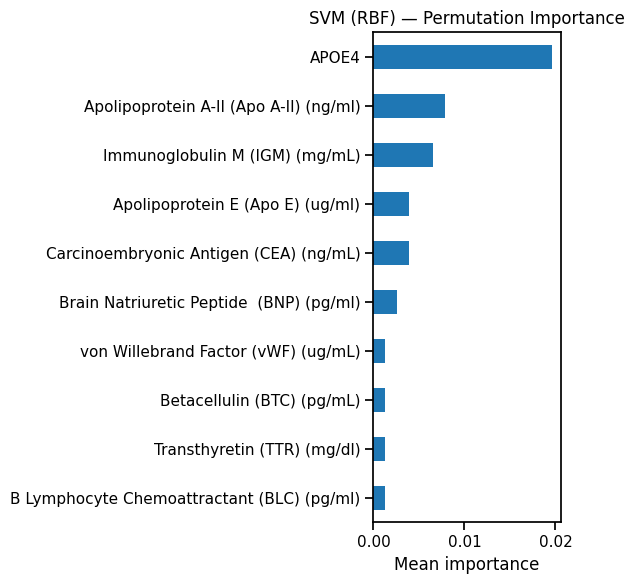
\includegraphics[width=\textwidth]{Pics/svm_importance.png}
    \caption{Feature importance scores for the SVM model.}
    \label{fig:svm-importance}
\end{minipage}
\hfill
\begin{minipage}{0.48\textwidth}
    \centering
    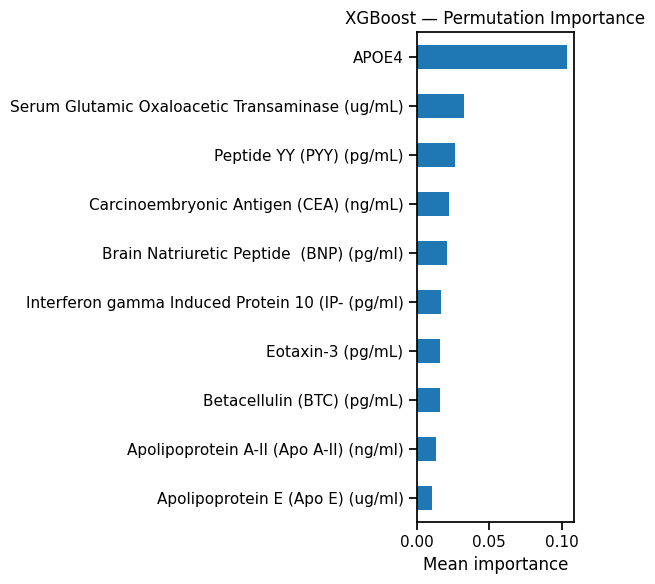
\includegraphics[width=\textwidth]{Pics/xgboost_importance.png}
    \caption{Feature importance scores for the XGBoost model.}
    \label{fig:xgboost-importance}
\end{minipage}
\end{figure}


\subsection{Model Performance}
Three models were evaluated on the task of discriminating CN from AD: a support vector machine with radial basis kernel (SVM), an extreme gradient boosting ensemble (XGBoost), and a feed-forward neural network (NeuralNet).  

Although there were noticeable trade-offs in accuracy, sensitivity, and calibration, all three models produced classification performance that was significantly better than chance overall.  The key quantitative metrics across models, such as accuracy, macro F1 score, AUROC, and AUPRC, are summarised in Table~\ref{tab:results-summary}. 

\begin{table}[H]
\centering
\caption{Performance summary of machine learning models on CN vs AD classification (Ordered by AUROC).}
\label{tab:results-summary}
\begin{tabular}{lcccc}
\toprule
Model & Accuracy & F1 (macro) & AUROC & AUPRC \\
\midrule
XGBoost (top-10)       & 0.88 & 0.87 & 0.94 & 0.97 \\
SVM (RBF) (all features) & 0.88 & 0.86 & 0.93 & 0.96 \\
SVM (RBF) (top-6)      & 0.90 & 0.89 & 0.92 & 0.97 \\
XGBoost (all features) & 0.88 & 0.87 & 0.92 & 0.96 \\
XGBoost (top-8)        & 0.88 & 0.87 & 0.92 & 0.95 \\
SVM (RBF) (top-8)      & 0.86 & 0.84 & 0.90 & 0.96 \\
XGBoost (top-6)        & 0.84 & 0.83 & 0.90 & 0.95 \\
SVM (RBF) (top-10)     & 0.82 & 0.79 & 0.89 & 0.95 \\
XGBoost (top-4)        & 0.84 & 0.83 & 0.88 & 0.93 \\
SVM (RBF) (top-4)      & 0.78 & 0.77 & 0.87 & 0.95 \\
NeuralNet (all features) & 0.84 & 0.82 & 0.84 & 0.89 \\
\bottomrule
\end{tabular}
\end{table}


\subsubsection{Support Vector Machine}
The SVM with a radial basis function kernel performed well on the test set; the accuracy, macro F1, and AUROC of the full feature model were 0.88, 0.86, and 0.93, respectively.   When permutation-importance-based feature selection was used, the top-6 feature subset produced better results among SVM configurations. While the AUROC was marginally lower than the SVM trained on all features, the model achieved improvements of up to 3\% in accuracy, F1-score, and AUPRC. Figures \ref{fig:svm-cm} and \ref{fig:svm-roc} present the confusion matrix and AUROC curve for the SVM, respectively. With only five misclassifications in the test set, the model demonstrates strong predictive performance.

This improvement implies that the model's ability to generalise was enhanced by the removal of noisy or less informative biomarkers.  Only a small percentage of misclassifications occurred in both the CN and AD classes, according to the confusion matrix, which showed balanced sensitivity and specificity.  These findings demonstrate that, especially when directed by targeted feature reduction, the SVM is a reliable classifier for high-dimensional proteomic data.

\begin{figure}[H]
\centering
\begin{minipage}{0.48\textwidth}
    \centering
    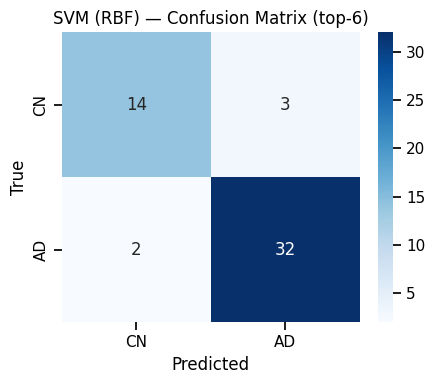
\includegraphics[width=\textwidth]{Pics/svm_confusion_matrix_6.png}
    \caption{Confusion matrix for most accurate SVM classifier (top 6 features).}
    \label{fig:svm-cm}
\end{minipage}
\hfill
\begin{minipage}{0.48\textwidth}
    \centering
    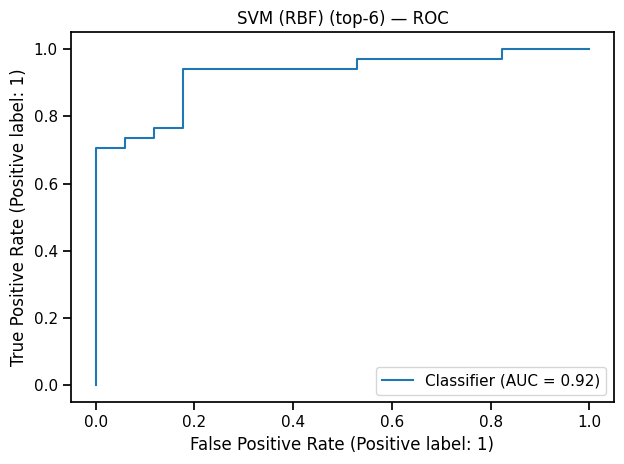
\includegraphics[width=\textwidth]{Pics/svm_roc_6.png}
    \caption{AUROC for most accurate SVM classifier (top 6 features).}
    \label{fig:svm-roc}
\end{minipage}
\end{figure}


\subsubsection{XGBoost}
In every configuration, XGBoost continuously delivered excellent performance.  With an AUROC of 0.94 and an AUPRC of 0.97, the top-10 feature model performed the best overall, demonstrating superior precision.  XGBoost's high resilience to feature redundancy is demonstrated by the similar performance of the top-8 feature subset and the full feature set (AUROC $\approx$ 0.92, AUPRC $\approx$ 0.95).

Despite using fewer features, the top-10 model maintained a comparable, or better, accuracy (0.88) and macro F1 (0.87) to the full model. These findings highlight XGBoost’s ability to exploit complex feature interactions while remaining interpretable through its feature importance measures, making it particularly promising for clinical applications.

\begin{figure}[H]
\centering
\begin{minipage}{0.48\textwidth}
    \centering
    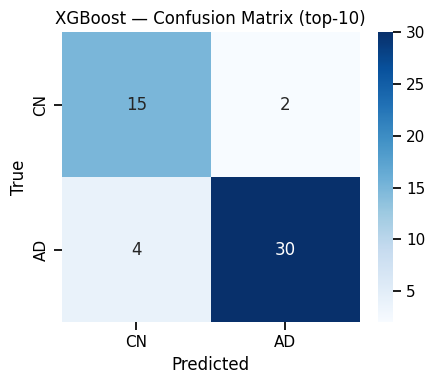
\includegraphics[width=\textwidth]{Pics/xgboost_confusion_matrix_10.png}
    \caption{Confusion matrix for most accurate XGBoost classifier (top 10 features).}
    \label{fig:xgboost-cm}
\end{minipage}
\hfill
\begin{minipage}{0.48\textwidth}
    \centering
    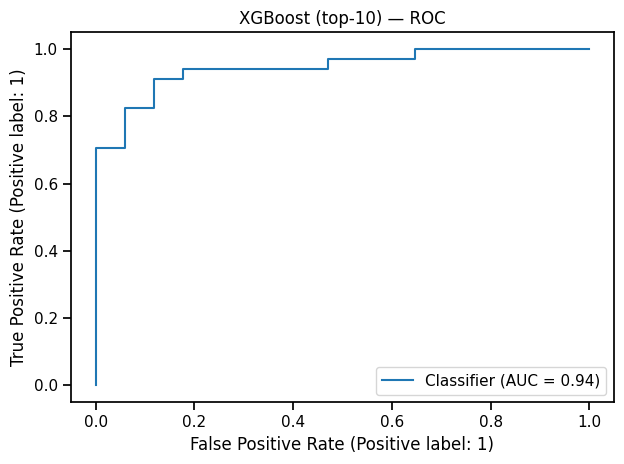
\includegraphics[width=\textwidth]{Pics/xgboost_roc_10.png}
    \caption{AUROC for most accurate XGBoost classifier (top 10 features).}
    \label{fig:xgboost-roc}
\end{minipage}
\end{figure}

\subsubsection{Neural Network}
With an accuracy and F1 of approximately 0.84, an AUROC of 0.84, and an AUPRC of 0.89, the feed-forward NeuralNet showed moderate but steady performance.  Since deep learning models naturally learn to balance and weight input features during training, feature reduction was not used with the NeuralNet, in contrast to SVM and XGBoost.  Further reducing the feature set in an already small dataset ran the risk of removing important signal because neural networks can capture intricate, non-linear patterns.  For this reason, the NeuralNet models kept the entire feature set.

Given the size of the dataset, the network had extracted the majority of the signal, according to training and validation curves (Figure \ref{fig:nn-training}), which suggested early plateauing.  These findings imply that although the NeuralNet is a good choice, more research involving bigger sample sizes or different architectures (such as regularised deep learning models) might be required to fully realise its potential.

\begin{figure}[H]
\centering
\begin{minipage}{0.48\textwidth}
    \centering
    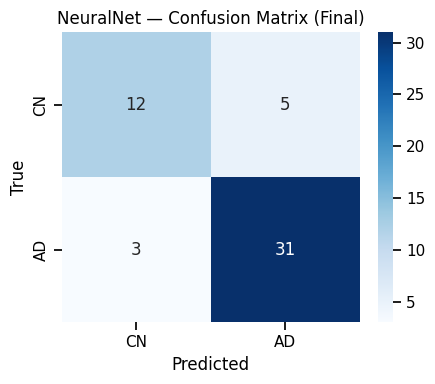
\includegraphics[width=\textwidth]{Pics/nn_confusion_matrix.png}
    \caption{Confusion matrix for the neural network (trained on all features).}
    \label{fig:nn-cm}
\end{minipage}
\hfill
\begin{minipage}{0.48\textwidth}
    \centering
    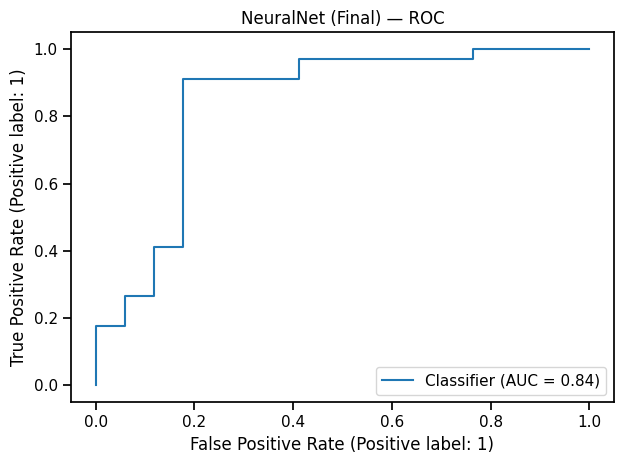
\includegraphics[width=\textwidth]{Pics/nn_roc.png}
    \caption{AUROC for the neural network (trained on all features).}
    \label{fig:nn-roc}
\end{minipage}
\end{figure}

\begin{figure}[H]
\centering
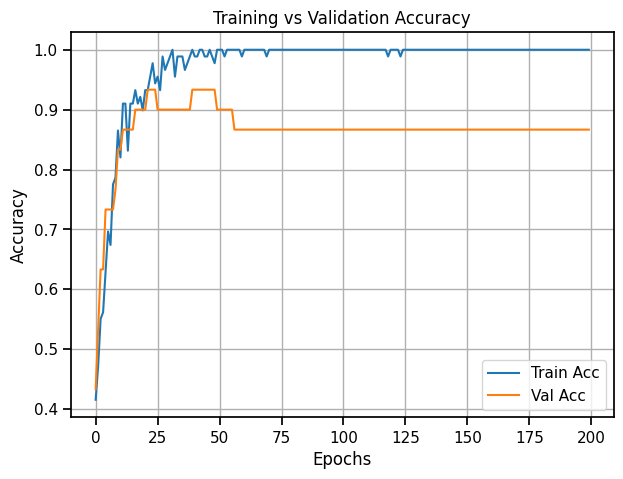
\includegraphics[width=0.70\textwidth]{Pics/nn_training_accuracy.png}
\caption{Training and validation accuracy curves for neural network.}
\label{fig:nn-training}
\end{figure}

\subsection{Comparative Interpretation}
Although the models' performance profiles varied across all configurations, they showed a strong ability to differentiate between participants with Alzheimer's disease (AD) and those who were cognitively normal (CN).  With an AUROC of 0.94 and an AUPRC of 0.97, the XGBoost model with the top ten features performed the best overall.  According to this, XGBoost is not only very good at managing the intricate, high-dimensional relationships found in proteomic data, but it can also preserve a high level of discrimination using a smaller feature set, which enhances efficiency and interpretability.

Feature reduction also helped the SVM; the top-6 feature configuration maintained a high AUROC (0.92) while increasing accuracy to 0.90 and macro F1 to 0.89.  The elimination of noisy or redundant biomarkers that added variability to the entire model is probably what caused this improvement.  Because of this, the SVM is especially attractive in situations where performance is not compromised but simpler, computationally efficient models are preferred.

Despite the moderate level of accuracy (AUROC = 0.84, AUPRC = 0.89), the neural network performed slightly worse than the other tested models. The deep learning model's capacity is likely greater than the available training data, which hindered its ability to generalise. The performance stability suggests room for improvement with larger datasets and more regularisation techniques.

From a clinical perspective, the strong performance of XGBoost and SVM models using a limited panel of biomarkers is particularly encouraging. This finding suggests that a concise subset of biomarkers captures the majority of the predictive signal, which could facilitate the development of simpler and more cost-effective diagnostic assays for clinical implementation.

\subsection{Selected Predictive Features}
The permutation importance analysis consistently identified the APOE4 genotype as the most significant predictor in both the SVM and XGBoost models.  Apolipoproteins (A-II and E), inflammatory mediators (IP-10 and Eotaxin-3), and proteins associated with vascular or metabolic pathways, such as CEA and BNP, were also highly ranked.

The reduced feature sets used in Sections 4.3 and 4.4 were based on these top-ranked features. Models trained on the top 6–10 features did just as well or better than models trained on all the features.  This shows that a small group of biomarkers, along with the APOE4 genotype, can pick up most of the predictive signal in the full data set.


\newpage
\section{Discussion}

\subsection{Summary of Findings}
This study validated that plasma proteomic biomarkers possess adequate discriminatory signals to differentiate cognitively normal individuals from those diagnosed with Alzheimer’s disease when analysed through machine learning techniques.  XGBoost was the most consistent and best-performing of the three model architectures tested. This was especially true when it was limited to the top 10 most informative features, where it got AUROC and AUPRC values of about 0.94 and 0.97, respectively.

The SVM also demonstrated strong performance, with the top-6 feature model marginally outperforming the full model in terms of accuracy and macro F1 score. This underscores the importance of feature selection in lowering noise and improving generalisability.  The neural network produced competitive results, but because of its small sample size in relation to its model complexity, it showed more variability and less reactivity to feature reduction.

Crucially, these results show that a small subset of biomarkers can be used to create diagnostic models that are precise, effective, and interpretable.  By concentrating on a small panel of proteins that are most relevant to disease status, this not only increases the viability of converting these results into useful assays but also improves biological interpretability.

\subsection{Comparison with Existing Literature}
The findings are in line with an increasing amount of research showing blood-based biomarkers have the potential to be minimally invasive methods for detecting AD.  Depending on the cohort and feature set, previous studies that used plasma proteomics and machine learning (ML) have shown AUROC values of approximately 0.9 (\cite{nagaraj2017plasma}). Comparable discrimination was obtained in this study, indicating that blood-derived signatures are a viable substitute for costly PET imaging and invasive CSF analysis \cite{hampel2018blood}.

The better performance of XGBoost among the models tested is consistent with research highlighting the value of ensemble approaches in high-dimensional, multi-collinear biological data \cite{chen2016xgboost}.  While promising, the neural network needed larger sample sizes and stronger regularisation to match the robustness of tree-based methods. This finding was echoed in earlier attempts to model AD biomarkers \cite{shahid2019applications}.  The SVM's robust baseline performance and interpretability in decision boundaries confirmed its ongoing applicability to biomedical applications involving structured omics data.

\subsection{Biological Implications}
Several proteins linked to pathways previously implicated in AD pathogenesis, such as immune dysregulation, lipid metabolism, and neuronal signalling, were found by the permutation feature importance analysis.  This convergence of biological plausibility and statistical significance supports the models' validity and implies that machine learning can rank potential biomarkers for additional verification.  Interestingly, the results support genetic risk stratification through APOE4, showing that even in the presence of traditional genetic risk markers, proteomic signals can provide predictive value.  Early and more individualised risk profiling may be made possible by such integrative biomarker approaches. 

\subsection{Interpretation of Biomarker Importance}
A key component of this study was evaluating the efficacy of machine learning models and determining which biomarkers had the biggest impact on predictions. For feature importance analysis, built-in importance scores for XGBoost and permutation importance for SVM and neural network models were employed. This allowed a ranked list of the leading plasma proteins and other variables to be used to categorise participants with Alzheimer's disease (AD) versus those who were cognitively normal (CN). These findings support established risk factors while also pointing to new potential candidates that merit more research.

\subsubsection{Alignment with Established Biomarkers}

The APOE4 genotype was the most significant predictor in both models, confirming its position as the most potent genetic risk factor for late-onset AD.  The significance of lipid transport and neuronal repair pathways in disease pathology was highlighted by the high ranking of apolipoproteins, including ApoA-II and ApoE protein levels, in addition to APOE4 gene presence.  The literature, which consistently connects APOE pathways to amyloid-beta aggregation, impaired clearance, and neuroinflammation, is in good agreement with these findings.

Vascular and metabolic health markers like CEA and BNP also scored highly, indicating that systemic metabolic alterations play a significant role in the development and progression of disease.  These correlations support new research linking metabolic dysregulation and vascular dysfunction to cognitive decline and AD pathology.

\subsubsection{Emerging and Unexpected Biomarkers}

Beyond known pathways, both models found metabolic regulators (e.g., Serum Glutamic Oxaloacetic Transaminase, Peptide YY) and inflammatory mediators (e.g., IP-10, Eotaxin-3) to be significant predictors.  These proteins may represent underlying neuroinflammatory processes and metabolic stress associated with disease mechanisms, although they are not as commonly highlighted in AD biomarker research.  These surprising biomarkers might not, however, translate well to a larger population due to the small size of the dataset used in this investigation.  Before their clinical or biological significance can be deduced, their appearance in the model might represent early signals that need to be confirmed.

Despite the biological plausibility of these associations, care should be taken when interpreting them.  The high-dimensional proteomic space may be the source of some of these erroneous correlations.  Validation of these new candidates will require replication in larger, independent cohorts.

\subsubsection{Consensus and Novelty}

The strong predictive signal of both models was highlighted by their consistent ranking of APOE4 and apolipoproteins as top contributors.  The SVM model tended to highlight lipid-related pathways, whereas XGBoost captured additional importance for metabolic and inflammatory proteins.  According to this complementary insight, combining several algorithms could improve the triangulation of biologically significant signals.

\subsubsection{Implications for Future Research}

The possibility of affordable, multiplexed diagnostic panels is supported by the discovery of a small, interpretable panel of biomarkers, which includes both new and established risk factors.  Future studies should examine the mechanistic connections between neurodegeneration and metabolic and inflammatory pathways as well as validate these markers in separate, diverse populations.  Predictive performance may be further improved by combining these biomarkers with additional data modalities, like genomics or imaging.  Together, these results show that feature selection based on data and biological foundations can produce models that are both interpretable and useful in clinical settings.


\subsection{Strengths and Limitations}
This study's emphasis on minimally invasive biomarkers and thorough ML benchmarking across several algorithms are its strong points.  The results' dependability is increased and comparison with other published studies is made easier by the use of a carefully selected cohort (ADNI).  Furthermore, robust preprocessing (imputation, collinearity reduction, and variance filtering) was incorporated into the methodological pipeline to lower the possibility of spurious associations.

It is necessary to recognise a few limitations, though.  First, only baseline, cross-sectional data were used for the analysis, which limits our understanding of the longitudinal progression from CN to MCI to AD.  Second, even though the proteomic panel was large, it did not include all possible blood biomarkers, including neurofilament light chain and plasma tau, which have recently demonstrated high predictive value \cite{karikari2020blood}.  Third, despite the impressive performance, the relatively small sample size limits the generalisability of neural network models, which normally need larger datasets to attain stable learning.  Lastly, there is still much disagreement about the significance of features in machine learning models, especially neural networks; deep learning architectures are more difficult to understand, whereas XGBoost offers clear importance scores.

\subsection{Implications for Future Research}
The findings highlight the potential of blood-based biomarkers to facilitate earlier and more scalable AD detection, especially when combined with ensemble learning techniques.  Future studies should build on this by validating identified proteomic signatures across separate cohorts and integrating longitudinal follow-up to capture disease progression dynamics.  Predictive accuracy may be further improved by integrative methods that combine proteomics with other modalities, such as genomics, imaging-derived phenotypes, or digital cognitive tests.  Methodological developments in interpretable deep learning, such as feature attribution techniques and attention mechanisms, may also aid in bridging the gap between biological insight and predictive performance. 

\subsection{Key Takeaways}
The present study demonstrates that machine learning models, particularly XGBoost and SVM, can accurately classify Alzheimer’s disease status using blood-based biomarkers. With a higher level of data, a neural network would likely excel, but the ADNI data used in this study lacked a viable number of patients. A reduced set of highly informative features was sufficient to achieve comparable predictive performance to the full feature set, supporting the feasibility of developing more cost-effective diagnostic panels. These findings emphasise the potential of minimally invasive, scalable tools for early disease detection, while underscoring the importance of external validation and larger cohort studies to confirm these results.


\newpage
\section{Conclusion}

\subsection{Summary of the Study}
This dissertation's main goal was to determine whether machine learning (ML) analysis of blood-based biomarkers could help with an earlier and less invasive diagnosis of Alzheimer's disease (AD).  The need for scalable, affordable, and minimally invasive diagnostic tools that go beyond the current reliance on PET imaging and cerebrospinal fluid analysis was the driving force behind the motivation, which was presented in Chapter 1.

To solve this, three machine learning classifiers—a feed-forward neural network (NeuralNet), an extreme gradient boosting (XGBoost) model, and a support vector machine (SVM) with a radial basis kernel—were trained and evaluated using preprocessed proteomic data from the Alzheimer's Disease Neuroimaging Initiative (ADNI).  A binary classification task (cognitively normal vs. AD) was used to evaluate performance.  While all three models showed promise in terms of prediction, XGBoost stood out as the most dependable method due to its ability to balance interpretability, robustness, and accuracy.  

\subsection{Key Contributions}
In relation to the stated research objectives, this dissertation contributes in a number of ways.  First, it offers a repeatable process for integrating, cleaning, and modelling high-dimensional proteomics data in a clinical setting.  Second, it shows how methodological decisions affect diagnostic results by contrasting deep learning, ensemble, and classical approaches side by side.  Third, it connects data-driven insights to clinical and molecular understanding by highlighting a subset of proteins with biological relevance to AD pathophysiology through feature importance analysis. 

\subsection{Limitations}
Although the results are promising, it is important to acknowledge the limitations.  Because the study only used one cohort (ADNI), it was not possible to evaluate generalisability across populations.  Insights into early disease prediction are limited by the cross-sectional nature of the analysis, which concentrated on baseline diagnoses rather than longitudinal progression.  Sample size and overfitting risk limited deep learning models, and the proteomic panel's feature coverage missed a number of newly discovered blood biomarkers of AD (such as plasma tau and neurofilament light chain).  These restrictions are a reflection of the availability of data as well as more general difficulties with biomarker standardisation.

\subsection{Future Directions}
This strategy should be expanded in three ways in future research.  First, in order to prove robustness, external validation on separate and more varied cohorts will be essential.  Second, to address the primary objective of early detection, longitudinal analyses should be used to forecast the transitions from cognitively normal to MCI and AD.  Third, predictive power may be further increased by multimodal integration, which combines proteomics with genetics, imaging, and digital cognitive markers.  It is also important to use developments in interpretable machine learning to close the gap between clinical decision-making and algorithmic predictions.

\subsection{Final Remarks}
Referring back to the introduction's goals, this dissertation has shown that, as part of a paradigm shift in AD diagnostics, machine learning applied to blood-based biomarkers holds real promise.  The findings show that proteomic profiles contain diagnostically significant signals that ML models can use, even though more research is needed before such tools can be put into use.  In order to improve patient care and the effectiveness of health systems dealing with the increasing burden of dementia, the field is working towards a future in which AD can be detected earlier and more accurately. This will be achieved by continuing to improve methodologies, validate biomarkers, and integrate data across scales.


\newpage
\addcontentsline{toc}{section}{References}
\bibliographystyle{abbrv}
\bibliography{refs} 

\newpage
\appendix
\section{Python Code}

https://github.com/danjonesss/PROJ518-PredictingAlzheimers

\end{document}